\documentclass[border=8pt,tikz]{standalone}
\usepackage{amsmath,amssymb}
\usepackage{tikz}
\usetikzlibrary{arrows.meta,calc,decorations.pathreplacing,patterns,shapes.geometric,positioning,shadings,plotmarks}

\begin{document}
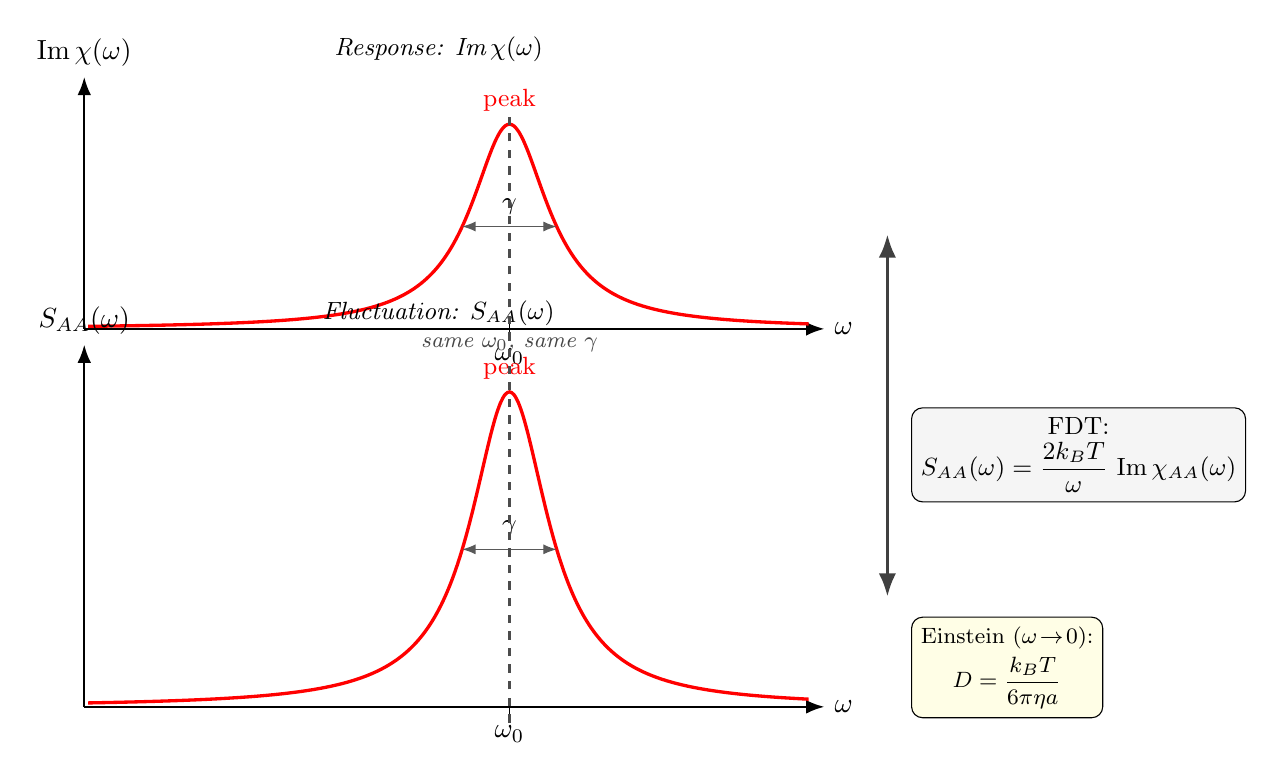
\begin{tikzpicture}[>=Latex]

% =====================================================================
% Layout parameters
% Two stacked plots sharing the same horizontal axis (omega).
% Top: Im chi(omega) -- response / absorption
% Bottom: S(omega)   -- equilibrium fluctuation power spectrum
%
% Lorentzian: L(w; w0, gamma) = (gamma/2)^2 / ( (w-w0)^2 + (gamma/2)^2 )
% Same w0, gamma for both peaks.
% Top peak height A1 = 1
% Bottom peak height A2 = (2 kT / w0) * A1 with chosen ratio = 1.6
% =====================================================================

\def\xL{0}
\def\xR{9}
\def\w0{5.4}        % resonance frequency
\def\gam{1.2}       % full width gamma
\def\hg{0.6}        % half width gamma/2
\def\peakA{2.6}     % top peak height (chi'')
\def\peakB{4.0}     % bottom peak height (S) -- ratio ~ 1.54 = 2kT/omega0

% ---------- Top axes: Im chi(omega) ----------
\begin{scope}[yshift=4.6cm]

  % axes
  \draw[->,thick] (\xL,0) -- (\xR+0.4,0) node[right] {$\omega$};
  \draw[->,thick] (\xL,0) -- (\xL,3.2) node[above] {$\operatorname{Im}\chi(\omega)$};

  % Lorentzian curve (Im chi)
  \draw[red,very thick,smooth,samples=160,domain=\xL+0.05:\xR+0.2]
        plot (\x, {\peakA*((\hg)*(\hg))/(((\x-\w0))*((\x-\w0)) + (\hg)*(\hg))});

  % omega_0 tick on axis
  \draw[thin] (\w0,0.06) -- (\w0,-0.12) node[below] {$\omega_0$};

  % gamma width indicator at half maximum (height = peakA/2)
  \pgfmathsetmacro{\halfA}{\peakA/2}
  \draw[<->,thin,gray!70!black]
        ({\w0-\hg},\halfA) -- ({\w0+\hg},\halfA)
        node[midway,above=1pt,black,font=\small] {$\gamma$};

  % peak top label
  \node[red,font=\small,above=1pt] at (\w0,\peakA) {peak};

  % title above top plot
  \node[font=\small\itshape] at (\xR/2,3.55) {Response: Im\,$\chi(\omega)$};

\end{scope}

% ---------- Bottom axes: S_AA(omega) ----------
\begin{scope}[yshift=-0.2cm]

  % axes
  \draw[->,thick] (\xL,0) -- (\xR+0.4,0) node[right] {$\omega$};
  \draw[->,thick] (\xL,0) -- (\xL,4.6) node[above] {$S_{AA}(\omega)$};

  % Lorentzian curve (S)
  \draw[red,very thick,smooth,samples=160,domain=\xL+0.05:\xR+0.2]
        plot (\x, {\peakB*((\hg)*(\hg))/(((\x-\w0))*((\x-\w0)) + (\hg)*(\hg))});

  % omega_0 tick on axis
  \draw[thin] (\w0,0.06) -- (\w0,-0.12) node[below] {$\omega_0$};

  % gamma width indicator at half maximum
  \pgfmathsetmacro{\halfB}{\peakB/2}
  \draw[<->,thin,gray!70!black]
        ({\w0-\hg},\halfB) -- ({\w0+\hg},\halfB)
        node[midway,above=1pt,black,font=\small] {$\gamma$};

  % peak top label
  \node[red,font=\small,above=1pt] at (\w0,\peakB) {peak};

  % title below bottom plot
  \node[font=\small\itshape] at (\xR/2,5.0) {Fluctuation: $S_{AA}(\omega)$};

\end{scope}

% ---------- Vertical dashed line connecting the two peaks ----------
% Top peak top in figure coords: (w0, peakA + 4.6)
% Bottom peak top in figure coords: (w0, peakB - 0.2)
\draw[dashed,gray!60!black,thick]
      (\w0,-0.4) -- (\w0,4.6+\peakA+0.2);

% ---------- FDT relation arrow + label between the two plots ----------
% Place an arrow from top axis to bottom axis at right side
\draw[<->,very thick,gray!50!black]
      (\xR+1.2,4.6+1.2) -- (\xR+1.2,1.2);

\node[draw,rounded corners,fill=gray!8,align=center,font=\small,
      anchor=west] at (\xR+1.5,3.0)
   {FDT: \\[2pt]
    $\displaystyle S_{AA}(\omega)=\frac{2k_BT}{\omega}\,\operatorname{Im}\chi_{AA}(\omega)$};

% ---------- Einstein DC-limit box (lower right) ----------
\node[draw,rounded corners,fill=yellow!10,align=center,
      font=\footnotesize,anchor=west] at (\xR+1.5,0.3)
   {Einstein ($\omega\!\to\!0$): \\[2pt]
    $\displaystyle D=\dfrac{k_BT}{6\pi\eta a}$};

% ---------- Annotation: peak positions match ----------
\node[gray!55!black,font=\footnotesize] at (\w0,4.4)
   {\textit{same $\omega_0$, same $\gamma$}};

\end{tikzpicture}
\end{document}
